\documentclass[12pt, a4paper]{article}
\usepackage{scrextend}
\usepackage{titlesec}
\usepackage{graphicx}
\usepackage{amsmath}
\usepackage{amsfonts} % for the real number symbol
\usepackage{geometry}
\usepackage[unicode]{hyperref}
\usepackage{titlesec}
\usepackage{titletoc}
\usepackage[sorting=none]{biblatex}
\usepackage{xurl}
\usepackage{enumitem}
\usepackage{indentfirst}
\numberwithin{equation}{section} % number equations by section
\renewcommand{\figurename}{Att.}
\renewcommand{\contentsname}{Saturs}
\renewcommand{\labelenumi}{\arabic{enumi})} % lists with 1)
\setlist{nosep}
\parindent=1cm
\linespread{1.213} % equivalent to 1.5 in word, experimentally.
\addbibresource{refs.bib}

\geometry{
    a4paper,
    lmargin=30mm,
    rmargin=20mm,
    tmargin=20mm,
    bmargin=20mm
}


\titleformat{\section}
    {\normalfont\large\bfseries}{\thesection . }{0.2em}{\MakeUppercase}
\titleformat{\subsection}
    {\normalfont\large\bfseries}{\thesubsection . }{0.2em}{}
\titleformat{\subsubsection}
    {\normalfont\normalsize\bfseries\itshape}{\thesubsubsection . }{0.2em}{}
\titlespacing*{\subsubsection}{0pt}{6pt}{0pt}

\begin{document}
\begin{titlepage}
    \begin{center}
        \vspace*{3cm}
        
        LATVIJAS UNIVERSITĀTE

        DATORIKAS FAKULTĀTE

        \vspace*{4cm}

        \large\textbf{COVID-19 IEROBEŽOŠANAS PROJEKTU PĀRVALDĪBAS ASPEKTI}
        
        \vspace{2cm}
        \normalsize{REFERĀTS IT PROJEKTU PĀRVALDĪBĀ}
         
             
    \end{center}
    \vspace{3cm}
    \begin{addmargin}[18em]{0em}
    Autors: \textbf{Pēteris Račinskis}
    \end{addmargin}

    \begin{addmargin}[18em]{0em}
    \hspace{1cm} Stud. apl. Nr. pr20015
    \end{addmargin}

         
    \vfill
    \begin{center}
    RĪGA 2022
    \end{center}
 \end{titlepage}
\newpage
\tableofcontents
\thispagestyle{empty}
\newpage
\setcounter{page}{3}


\section{Ievads}

ASFASFAF

\subsection{Darba mērķis un struktūra}

\newpage
\section{Otrā nodaļa --- ko šeit?}

\newpage
\section{Secinājumi}

Literatūras analīzē sniegts īss un nebūt ne pilnīgs --- vai vienlīdzīgi sadalīts --- līdz šim par atdarinošo mašīnmācīšanos veiktās pētnieciskās darbības pārskats. Jau izvēloties, par kurām tēmām rakstīts plašāk, par kurām --- mazāk detalizēti --- iespaidu uz darba saturu ir atstājusi motivējošās problēmas specifika. Tagad nepieciešams pie tās atgriezties un novērtēt, kas no visa nozarē pētītā un izgudrotā attiecas uz darba ievadā aprakstīto uzdevumu --- mešanas kustību iestrādāšanu atkritumu vai citu objektu pārvietošanā.

\subsection{Svarīgākās atziņas}

\begin{figure}[t!]
    \centering
    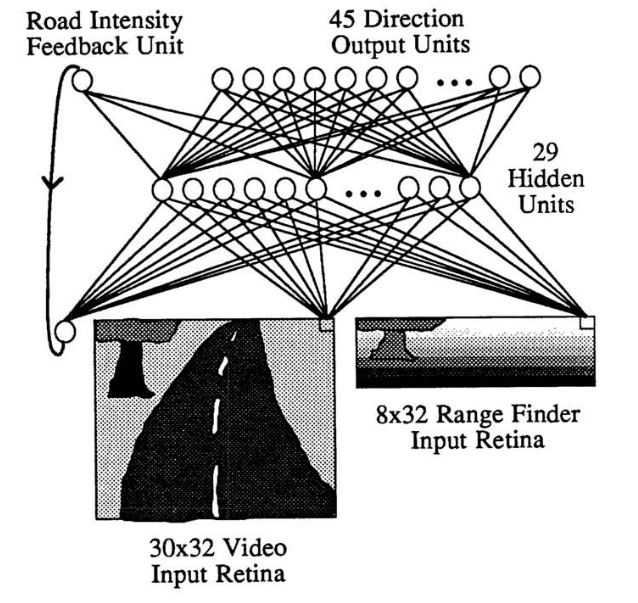
\includegraphics[height=6.8cm,page=1]{../img/alvinn_architecture.png}
    \caption{ALVINN modeļa uzbūve \cite{enc_stim}}
\end{figure}

\newpage
\addcontentsline{toc}{section}{Atsauces}
\printbibliography[title=Atsauces]

\end{document}